%======================================================================
\subsection{SIM-06 --- Built, 31 Oct: ParaView ready to view, background pictures, streamlines in the 3D view}\label{sec:sim06-pv-built}
%======================================================================

The three pieces you approved for the airflow results, in three commits, all Python (the module is
\file{src/Mod/BruceWorx/bruceworx\_cfd\_paraview.py}; ParaView 6.2.0 from \file{/Applications}, found by
\code{paraview\_app()}). ParaView cannot be embedded (its own Qt and VTK), so it only ever runs as a separate process.

\begin{figure}[!htbp]
\centering
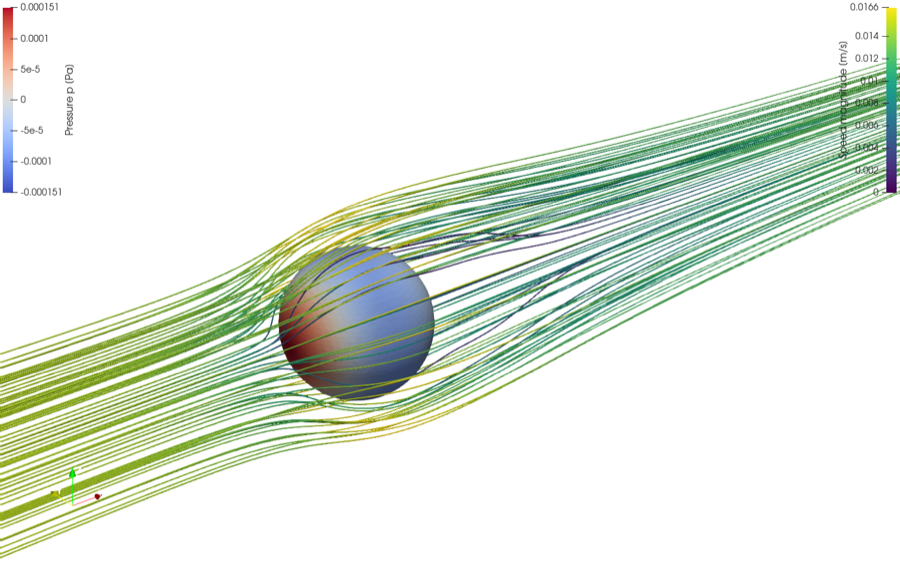
\includegraphics[width=0.49\linewidth]{fig/sim06pv_iso.png}\hfill
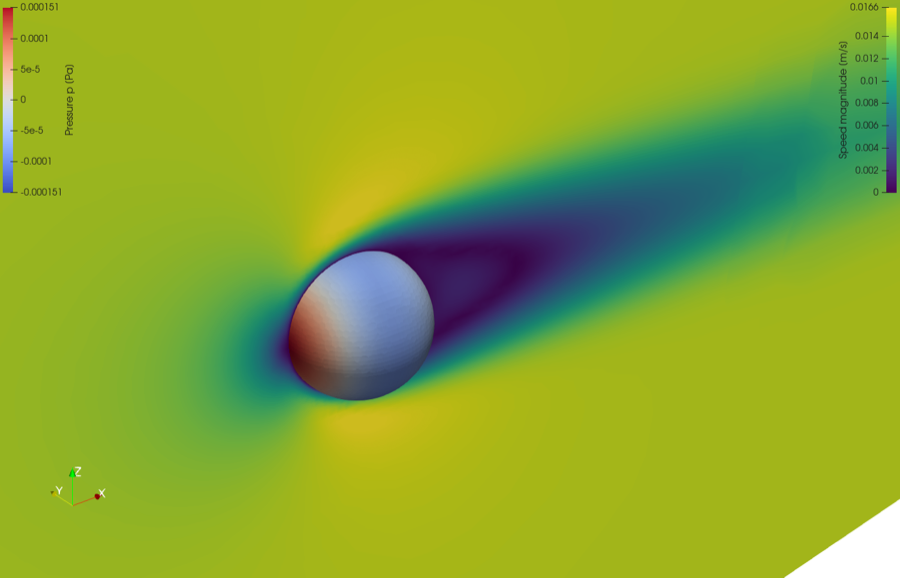
\includegraphics[width=0.49\linewidth]{fig/sim06pv_cut.png}
\caption{The background pictures of the 100\,mm ball study (laminar, 15\,mm/s, 2$^\circ$; 130\,000 cells), made by
\code{pvbatch} with no window in 3\,s. Left: isometric view, pressure on the part (blue--red about zero, in Pa) and 80
streamlines coloured by speed; right: the mid cut plane coloured by $|U|$ with the part. Both legends carry units.}
\label{fig:sim06pv}
\end{figure}

\paragraph{What you can do now.}
\begin{itemize}[nosep]
  \item \textbf{Open in ParaView} no longer opens an empty session. It writes \file{<case>/paraview/view.py} and starts
        ParaView with \code{--script}: the volume and the part patches loaded (foamToVTK output when it exists, else the
        OpenFOAM reader on \file{case.foam}, latest time), the surface pressure on the parts in Pa (OpenFOAM's $p$ is
        kinematic, so the script multiplies by $\rho$ of the study) on a blue--white--red map that is symmetric about
        zero, a mid XZ cut plane coloured by $|U|$ (viridis, 0 to the 99.5th percentile, so a wild wall cell does not
        flatten it), streamlines drawn as thin tubes, an isometric camera that frames the body with room for the wake, and
        two legends (``Pressure p [Pa]'', ``Speed magnitude [m/s]''). The script stays on disk to edit and re-run.
  \item \textbf{Where the streamlines start.} External flow: one point cloud upstream of the body, as wide as the body and
        wholly in front of it. Prop wash: one cloud above each disk (on the side the air is drawn from, 0.3\,$D$ up the
        thrust axis, radius 0.6\,$D$); the 3D view and ParaView use the same placement (\code{seed\_plan}).
  \item \textbf{Pictures in the background.} When a run ends and ParaView is installed, a child \code{pvbatch} renders
        \file{pv\_iso.png}, \file{pv\_side.png} and \file{pv\_cut.png} (1400\,$\times$\,900) into \file{<case>/paraview/}
        from the same script (batch mode); the button \textbf{Pictures} does it on demand. The panel polls it with a
        timer (the window never waits), shows the picture under the buttons with an Isometric / Side / Cut plane
        chooser, and the study \textbf{Report} adds a ``Flow pictures'' subsection with whatever pictures exist.
  \item \textbf{Degrades.} Without ParaView the Pictures and Open buttons are greyed with the install hint as their
        tooltip, a render that was asked for anyway ends as ``unavailable'' with that text, a hung \code{pvbatch} is
        killed after 300\,s (``stopped''), a failed one reports the tail of \file{render.log}, and a case with no
        results yet says so. None of these raise.
  \item \textbf{Streamlines in Vector Labs.} The results panel has a \textbf{Streamlines} tick and a seed count
        (default 200). It traces with \code{vtkStreamTracer} (RK4/5, both ways, at most one cell per step) on the
        millimetre copy of the volume, writes \file{streamlines.vtp} beside it (point arrays \code{U} and \code{speed}),
        and adds it to the study as a \code{Fem::FemPostPipeline} coloured by \code{speed}. FEM's own pipeline does
        display line sets, with its colour bar, so no Part wire compound was needed. Changing the seed count replaces
        the object; unticking hides it.
\end{itemize}

\paragraph{Timings (streamlines, 200 seeds, M-series Mac).} The 130\,000-cell ball case (real snappyHexMesh tetrahedra,
384 lines, 34\,000 points): 1.2\,s in total (read of the mm copy 0.09\,s, tracing 1.05\,s). A synthetic field on
1\,080\,000 tetrahedra: 1.1\,s the first time (0.9\,s of it making the millimetre copy) and 0.19\,s again (read 0.11\,s,
tracing 0.07\,s). The trace time depends on how far the lines run through fine cells, so a real 1M-cell case with a
boundary layer will be slower than the synthetic one; the ball is the better guide, and I expect 2 to 4\,s there. The
tracing runs on the GUI thread behind a wait cursor; nothing is cached across seed counts.

\paragraph{Decided while building.}
\begin{itemize}[nosep]
  \item \textbf{One script, two modes.} \file{view.py} and \file{render.py} are the same text with \code{mode} set to
        gui or batch, so the pictures are exactly what the opened session shows (the cut plane is translucent in the
        GUI session and opaque in the cut picture; streamlines are left out of the cut picture).
  \item \textbf{Reader fallback goes through a file.} With only the OpenFOAM reader, ParaView 6's stream tracer read
        the time-dependent pipeline wrongly (speeds up to 0.125\,m/s in a 0.017\,m/s flow), so the script writes the
        merged volume once to \file{paraview/volume\_*.vtu} and traces from that, and it locks the colour range after
        the tubes are made (adding tubes had rescaled it). Cause not found.
  \item \textbf{Colour ranges are fixed in the script,} not autoscaled by the tubes: speed $0\ldots$ p99.5 of the cut,
        pressure symmetric about zero. The in-app pressure scale is the other session's piece.
  \item \textbf{pvbatch needs a window server on macOS} (it renders on a hidden window); it works from a logged-in
        session, which is the app's case. Headless over ssh would need an off-screen build of ParaView.
  \item Report pictures are copied beside \file{report.tex} as \file{fig\_pv\_*.png} (a path with a space, like
        \file{Vector Labs}, would break \verb|\includegraphics|), and a stale picture is removed when a case has none.
\end{itemize}

\paragraph{Tests.} \file{TestBruceWorxCfdParaView.py}, 21 tests in the GUI run (0 failures, 1 skipped:
the OpenFOAM-reader render, covered by the end-to-end study test): scripts parse as Python for external flow and
a four-disk prop wash and hold the tracer, the cut, the legends with units, only the part patches (the inlet left out);
seeds are in front of the body and over each disk; a fake \code{pvbatch} that sleeps is killed on the timeout, one
that exits 3 reports its output; no ParaView gives the install text; with ParaView, \code{pvbatch} makes three PNGs
of a synthetic case (signature, size, more than 50 colours); \code{vtkStreamTracer} on U $=(1,0,0.3)$ gives lines whose
$\mathrm{d}z/\mathrm{d}x$ is 0.3 and speed 1.044 everywhere, each starting in a seed cloud, also for the wash seeds;
a volume without $U$ is a clean error; GUI: the lines show in the 3D view coloured by \code{speed}, the tick / seed
count / replace cycle, the panel's picture appears after a background render, and the report source carries the
pictures. \code{TestBruceWorxCfd}: see the commit messages for the result of the final run.

\paragraph{Open questions for you.}
\begin{enumerate}[nosep]
  \item \textbf{Render pictures automatically after every run?} It does now when ParaView is installed (about 10\,s of
        one core after the run, not blocking). Say if you would rather have only the button.
  \item \textbf{A second picture set for prop wash} (a vertical cut through each disk pair, the wake isosurface at half
        the induced velocity)? The three views are generic; the hover wake would show better with a view along the thrust
        axis.
  \item \textbf{Tracing off the GUI thread?} At 1 to 4\,s it is a wait cursor; a QThread would need the VTK call to
        release the GIL (it does for most filters), which I have not measured.
\end{enumerate}

\paragraph{Your answers (1 Nov).} (1) Yes, pictures after every run. (2) Yes, a prop-wash set along the thrust axis.
(3) Move tracing off the GUI thread if it is slow on a real frame (measure on the ROB-03 case first).


\paragraph{Follow-up, 1 Nov.} Items 3 and 4 of your answers are built.
\begin{itemize}[nosep]
  \item \textbf{Pictures stay automatic} after every run (when ParaView is installed); unchanged.
  \item \textbf{Prop-wash picture set.} For a prop-wash study the three generic pictures are joined by four kinds (a case with $n$
        pairs of opposite disks gets $n$ cuts): \emph{Along the thrust axis} (camera on the wake side looking up the axis, through a plane
        of speed half a propeller diameter below the disks, the frame behind it); \emph{Vertical cut} through each pair of opposite
        disks (the plane holds the thrust axis and both disk centres, speed $|U|$ on it, the frame in front; pairs are found by
        mirroring each disk about the centroid of all disks; a single or unpaired disk is cut towards the centroid); and
        \emph{Wake surface}: the isosurface of $|U|$ at half the induced velocity $v_i$ (the mean of the disks' momentum-theory
        values, $v_i=\sqrt{T/2\rho A}$ with the ring area, $9.33$\,m/s for the ROB-03 frame, so $4.67$\,m/s), translucent blue. The
        same script serves the opened ParaView session (\file{view.py}) and \code{pvbatch} (\file{render.py}); the set is chosen by
        \code{picture\_kinds}. The panel's picture list and the report follow the study: seven pictures for the frame, with
        captions that name the disks and the iso speed; old pictures (also of kinds the case no longer makes) are cleared before a run
        and in the report folder. On the ROB-03 results (217\,139 cells) all seven pictures took 13.4\,s of \code{pvbatch}
        after \code{foamToVTK} (1.8\,s).
\end{itemize}
\begin{figure}[h]\centering
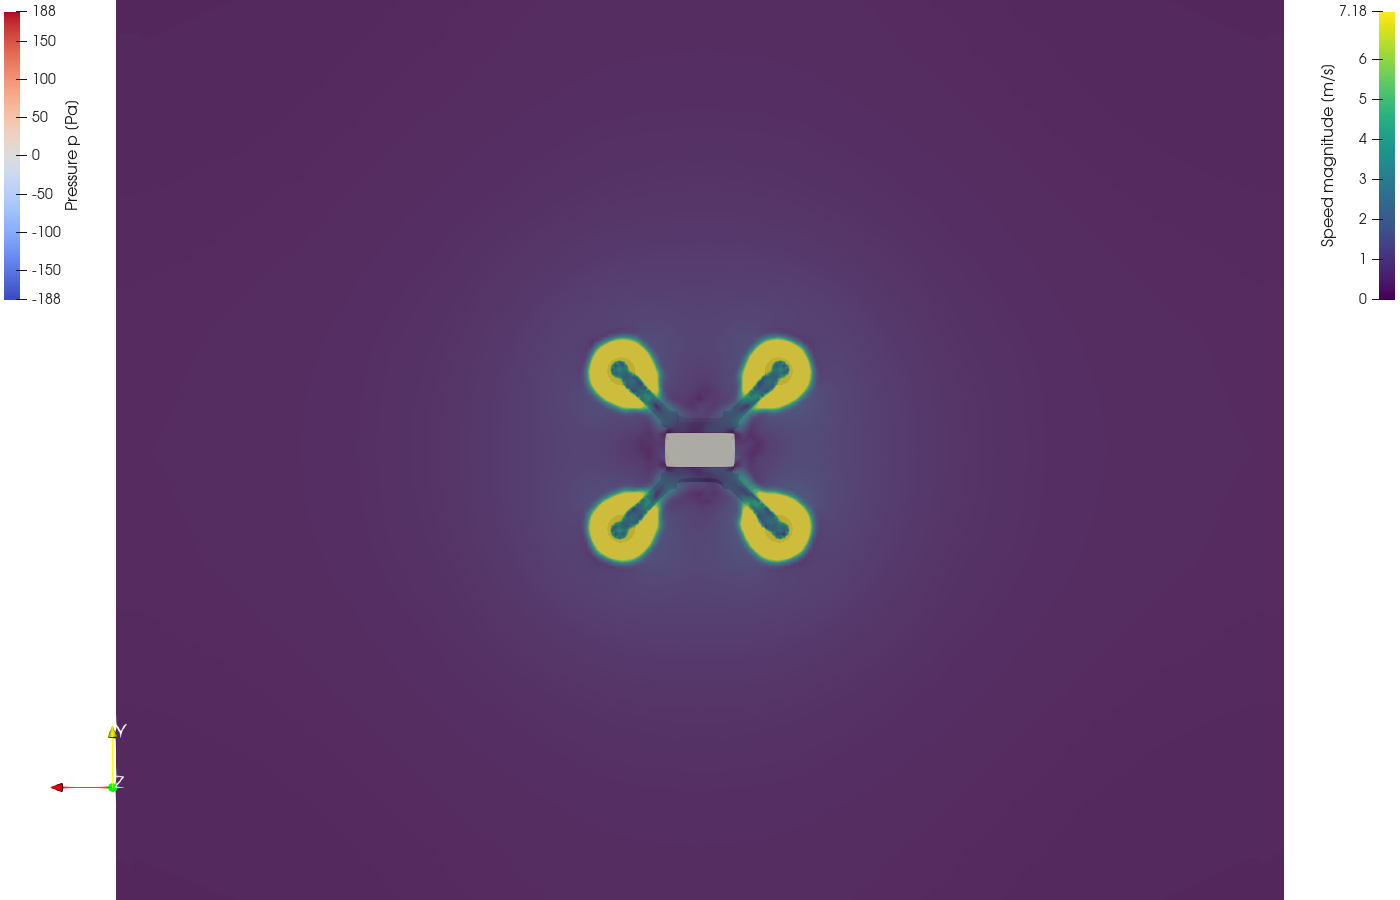
\includegraphics[width=0.32\linewidth]{fig/sim06_wash_axis.png}\hfill
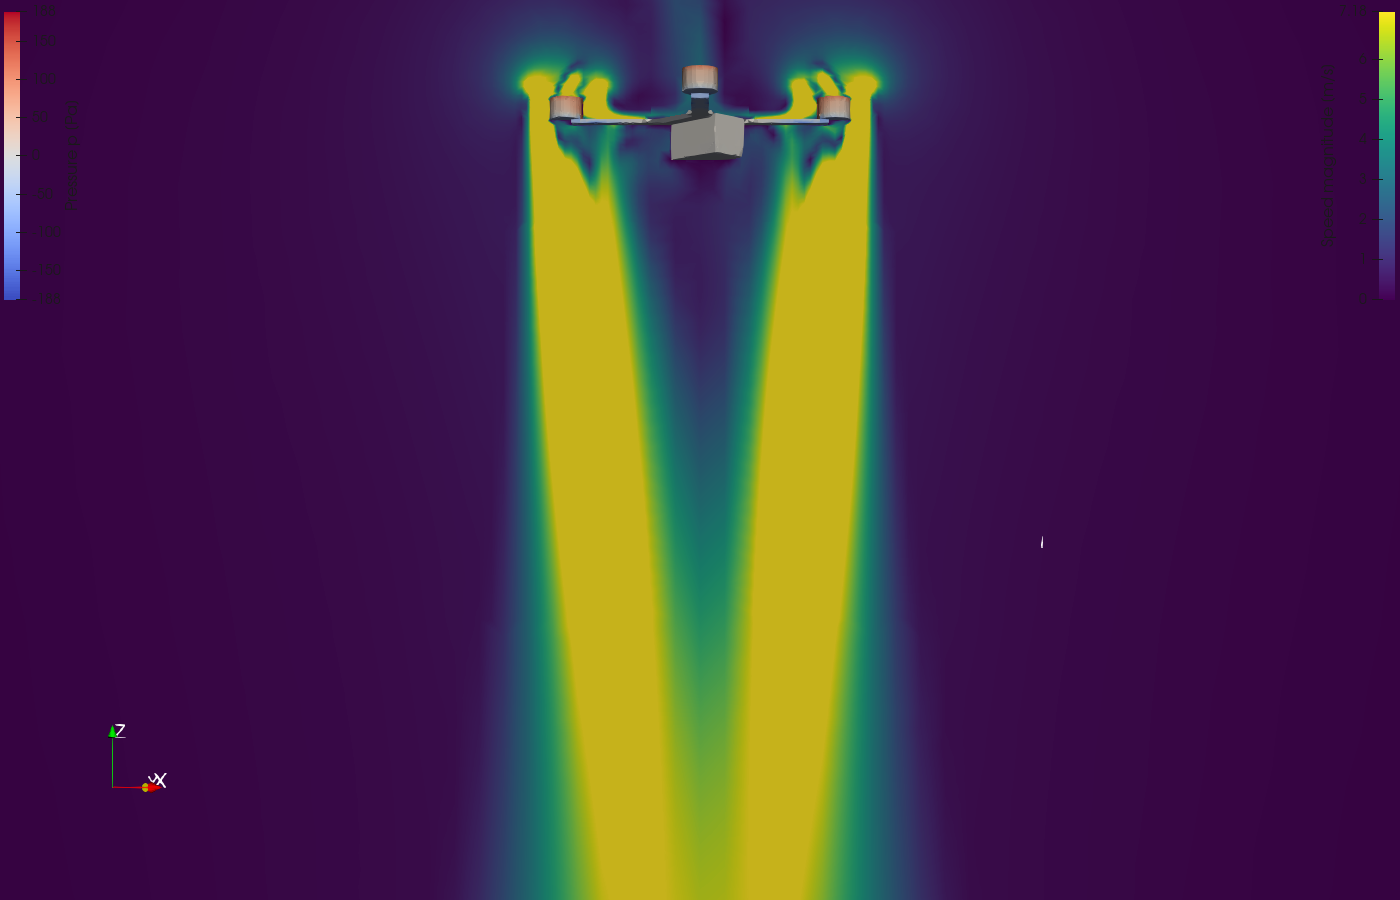
\includegraphics[width=0.32\linewidth]{fig/sim06_wash_cut1.png}\hfill
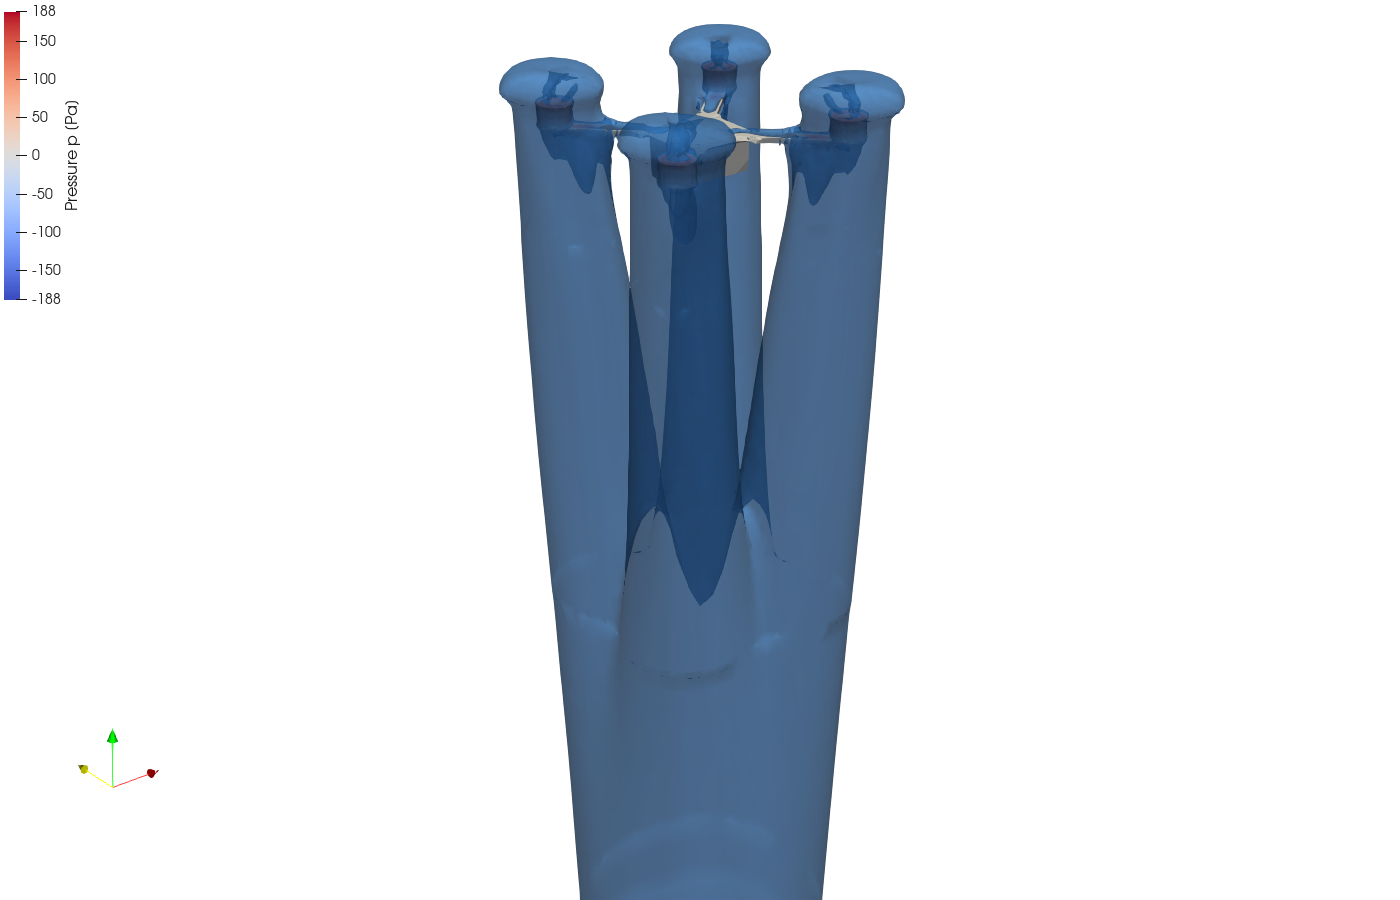
\includegraphics[width=0.32\linewidth]{fig/sim06_wash_wake.png}
\caption{ROB-03 frame, hover, four disks: along the thrust axis, a vertical cut through two opposite disks, the wake at half the
induced velocity.}
\end{figure}
\begin{itemize}[nosep]
  \item \textbf{Streamline tracing time, measured} on the ROB-03 frame result (217\,139 cells, 200 seeds, Apple silicon,
        \code{FreeCADCmd}, three runs): first time $3.5$\,s (making the millimetre copy $1.4$\,s, read $0.15$\,s, tracing $1.75$\,s);
        later $2.0$\,s ($1.73$\,s tracing, repeatable to $0.02$\,s); 50 seeds $0.9$\,s; 400 seeds $3.7$\,s. That is above the 2\,s
        line, and a thread cannot help: while a Python thread traced, the main thread was blocked for $1.9$\,s (200 seeds) and
        $3.3$\,s (400 seeds), the whole tracing time, because \code{vtkStreamTracer.Update} holds the GIL. So the tracing now runs in
        a \emph{worker process}: the app's own \file{bin/python3} (it has the VTK) runs \code{worker\_main}; the window polls it on a
        timer (\code{StreamJob}). The results panel shows ``Tracing streamlines from 200 seeds: 40\,\%'' and a \emph{Cancel}
        button; Cancel (or closing the panel, or changing the seed count) kills the worker. The seeds are traced in tenths because the
        tracer's own progress event never fires; the tenths cost nothing measurable ($4.2$\,s against $3.3$ to $4.0$\,s for 400
        seeds, the same 781 lines). The worker adds about $0.15$\,s of start-up (wall $2.34$\,s against $2.19$\,s in the process). The line
        object appears in the 3D view when the worker is done; ticking off while it runs hides it on arrival. Without a worker Python the old path
        (wait cursor, on the GUI thread) is used.
\end{itemize}
Tests added: the prop-wash picture kinds, pairs, plane normals and the iso speed ($2.5$ for $v_i=5$); the script carries the wash
configuration, the contour and \code{mag(U)} and none for external flow; pvbatch makes all seven pictures of a synthetic
wash case; the report copies the wash pictures and removes a stale one; the worker (done, progress never goes back, cancelled,
failed with a message); the panel traces in the background, shows the lines, and Cancel leaves no object.

\paragraph{Your answers (1 Nov, second round).} The wash pictures are named after the motors (``Cut through Motor~1 and
Motor~3''), not numbered pairs.
